\chapter{Perancangan}
\label{chap:Perancangan}

Pada bab 4 akan dibahas mengenai perancangan seperti kelas secara rinci dan perancangan antarmuka.

%Perancangan Kelas
\section{Perancangan Kelas}
\label{lab:Perancangan Kelas}
\hspace{0.5cm} Pada sub bab ini akan dibahas mengenai deskripsi kelas secara rinci pada aplikasi Pencari Rute Kendaraan Umum untuk Windows Phone. Untuk lebih jelas mengenai kelas yang ada pada aplikasi ini, penulis menyajikan gambar diagram kelas yang dapat dilihat pada  gambar ~\ref{fig:kelas}. 

% Kelas
\begin{figure}[h]
	\centering
		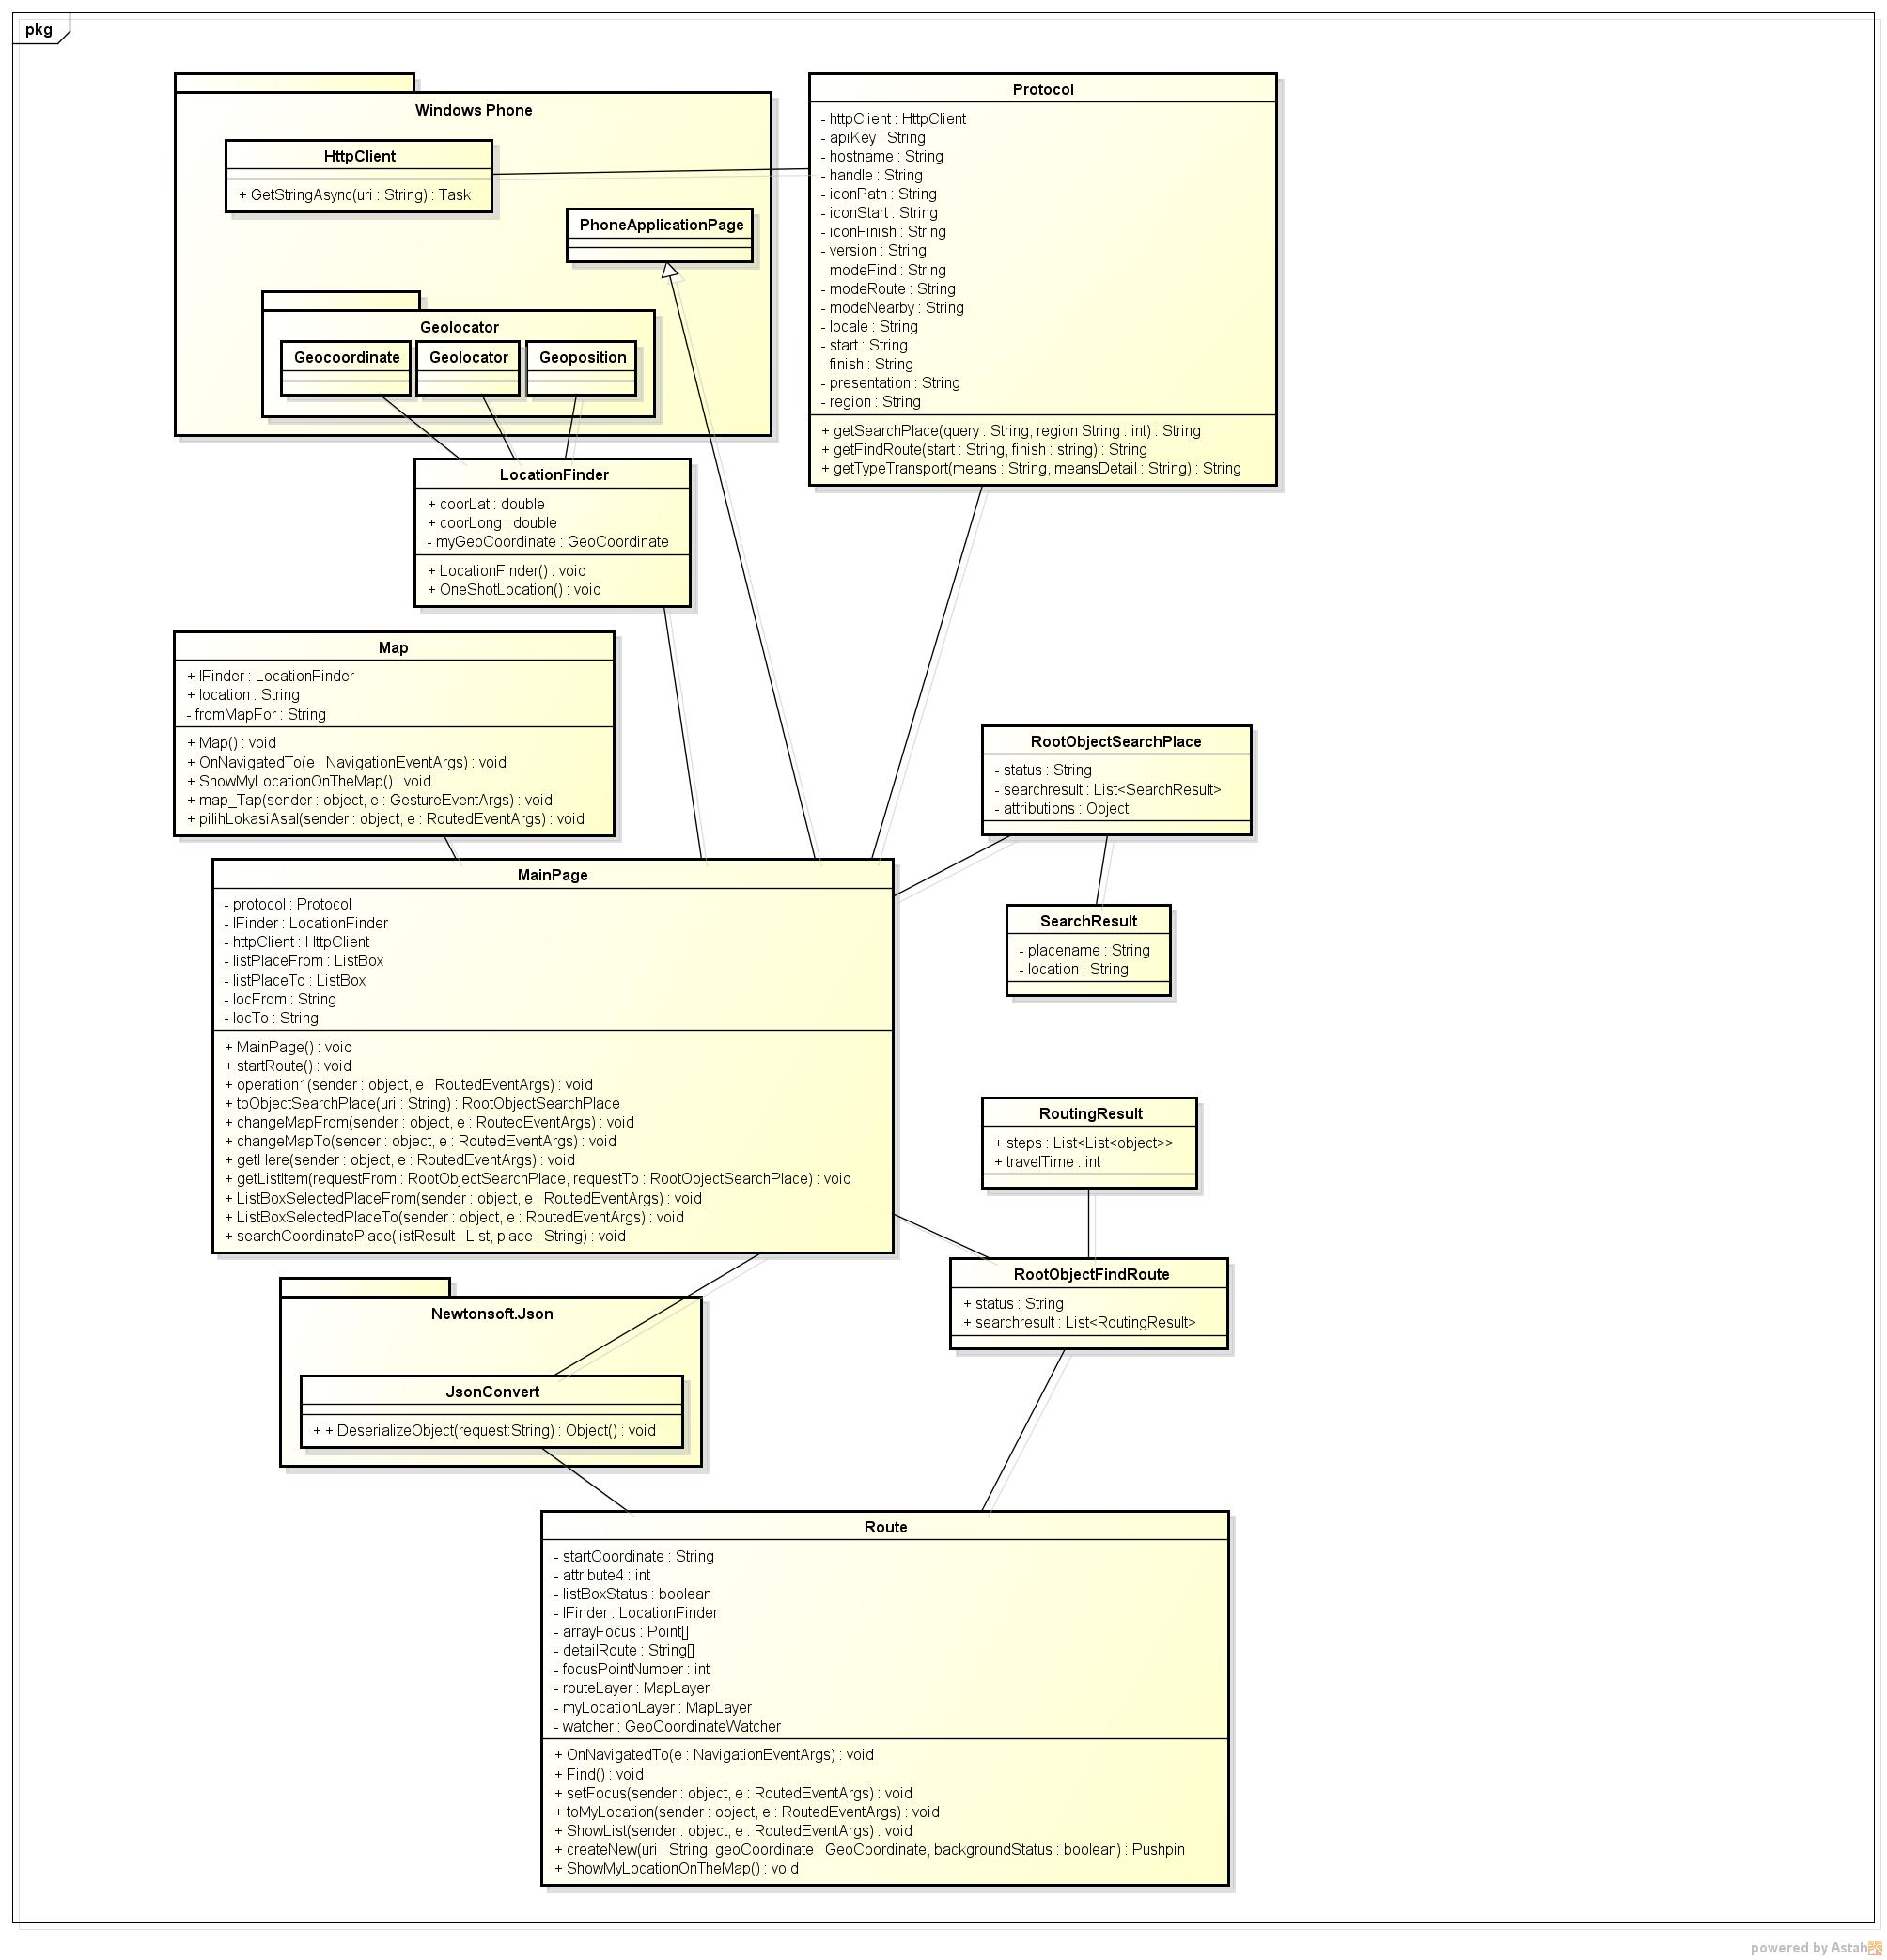
\includegraphics[scale=0.2]{Gambar/useCase_dan_Class/class4}
	\caption{Diagram Kelas}
	\label{fig:kelas}
\end{figure}

%Kelas PhoneApplicationPage
\subsection{Kelas \textit{PhoneApplicationPage}}
\label{lab:Kelas PhoneApplicationPage}
\hspace{0.5cm} \textit{PhoneApplicationPage} merupakan kelas bawaan Windows Phone yang menangani interksi pengguna dengan aplikasi dan siklus hidup aplikasi.

%Kelas MainPage
\subsection{Kelas \textit{MainPage}}
\label{lab:Kelas MainPage}
\hspace{0.5cm} \textit{MainPage} merupakan kelas kelas turunan dari kelas \textit{PhoneApplicationPage} yang menangani interaksi langsung antara halaman aplikasi dengan pengguna. Pada kelas ini akan ditaruh kontrol yang diperlukan. Berikut adalah penjelasan atribut-atribut yang dimiliki kelas ini:
\begin{enumerate}
	\item protocol bertipe Protocol untuk mendapatkan URL yang digunakan dalam permintaan ke Kiri API.
	\item lFinder bertipe LocationFinder yang akan menampung objek untuk pencarian lokasi.
	\item httpClient bertipe HttpClient merupakan objek yang akan mengurus permintaan dan kembalian dari Kiri API.
	\item listPlaceFrom bertipe ListBox untuk menampung dan menampilkan hasil pencarian lokasi terkait dari lokasi awal.
	\item listPlaceTo bertipe ListBox untuk menampung dan menampilkan hasil pencarian lokasi terkait dari lokasi tujuan
	\item locFrom bertipe string untuk menampung kordinat awal.
	\item locTo bertipe string untuk menampung kordinat tujuan.
\end{enumerate}

Berikut adalah penjelasan metode-metode yang dimiliki kelas ini:
\begin{enumerate}
	\item Metode MainPage digunakan sebagai konstruktor pada kelas MainPage. 
	\item startRoute digunakan untuk mendapatkan masukan pengguna lalu mengkalkulasi masukan tersebut menjadi kordinat asal dan tujuan lalu mengirimkannya ke kelas ShowRoute.
	\item toObjectSearchPlace digunakan untuk membuat objek RootObjectSearchPlace dengan masukan uri yang bertipe string.
	\item changeMapFrom digunakan untuk berpindah ke halaman mapFrom.
	\item changeMapTo digunakan untuk berpindah ke halaman mapTo.
	\item getHere digunakan untuk mendapatkan kordinat dimana perangkat berada.
	\item getListItem digunakan untuk membuat listBox lalu menampilkan ke pengguna. 
	\item ListBoxSelectedPlaceFrom digunakan untuk mendapatkan tempat asal yang dipilih pengguna.
	\item ListBoxSelectedPlaceTo digunakan untuk mendapatkan tempat tujuan yang dipilih pengguna.
	\item searchCoordinatePlace digunakan untuk mencari kordinat dari tempat pilihan pengguna.
\end{enumerate}

%Kelas Geocoordinate
\subsection{Kelas \textit{Geocoordinate}}
\label{lab:Kelas Geocoordinate}
\hspace{0.5cm} \textit{Geocoordinate} merupakan kelas bawaan dari Windows Phone yang akan dimanfaatkan untuk membaca \textit{latitude} dan \textit{altitude}.

%Kelas Geolocator
\subsection{Kelas \textit{Geolocator}}
\label{lab:Kelas Geolocator}
\hspace{0.5cm} \textit{Geolocator} merupakan kelas bawaan Windows Phone untuk mengkases lokasi. Dengan bantuan kelas ini maka dapat mengetahui status lokasi dari perangkat dan menemukan lokasi secara akurat.

%Kelas Geoposition
\subsection{Kelas \textit{Geoposition}}
\label{lab:Kelas Geoposition}
\hspace{0.5cm} \textit{Geoposition} merupakan kelas yang menampung lokasi sesuak kembalian \textit{Geolocator}.

%Kelas LocationFinder
\subsection{Kelas \textit{LocationFinder}}
\label{lab:Kelas LocationFinder}
\hspace{0.5cm} \textit{LocationFinder} merupakan kelas yang akan menampung lokasi perangkat. Berikut adalah penjelasan atribut-atribut yang dimiliki kelas ini:
\begin{enumerate}
	\item status bertipe \textit{boolean} sebagai penanda apakah GPS perangkat sudah siap.
	\item latitude bertipe long untuk menampung kordinat latitude.
	\item longitude bertipe long untuk menampung kordinat longitude.
\end{enumerate}

Berikut adalah penjelasan metode-metode yang dimiliki kelas ini:
\begin{enumerate}
	\item Metode onInit berfungsi untuk inisialisasi GPS perangkat dan memastikan bahwa GPS perangkat siap untuk menemukan lokasi.
	\item Metode getCoordinate berfungsi untuk mendapatkan kordinat latitude dan longitude dengan memanfaatkan kelas \textit{Geocoordinate}, \textit{Geolocator}, dan \textit{Geoposition}.   
\end{enumerate}

%Kelas PointFromMap
\subsection{Kelas \textit{PointFromMap}}
\label{lab:Kelas PointFromMap}
\hspace{0.5cm} \textit{PointFromMap} merupakan kelas yang akan mendapatkan titik yang ditunjuk pengguna pada peta lalu menerjemahkannya dalam bentuk titik kordinat. Berikut adalah penjelasan atribut-atribut yang dimiliki kelas ini:
\begin{enumerate}
	\item latitude
	\item longitude
\end{enumerate}

Berikut adalah penjelasan metode-metode yang dimiliki kelas ini:
\begin{enumerate}
	\item Metode getPoint berfungsi mengambil titik yang ditunjuk lalu menerjemahkan dalam bentuk latitude dan longitude. 
\end{enumerate}

%Kelas HttpClient
\subsection{Kelas \textit{HttpClient}}
\label{lab:Kelas HttpClient}
\hspace{0.5cm} \textit{HttpClient} merupakan kelas bawaan Windows Phone untuk mengatur pengiriman dan kembalian menggunakan protokol HTTP. Berikut adalah penjelasan metode-metode kelas \textit{HttpClient} yang dipakai untuk perancangan aplikasi ini:
\begin{enumerate}
	\item Metode GetStringAsync membutuhkan parameter alamat bertipe string dan mengembalikan kembalian dari Kiri dalam bentuk Task<string>.
\end{enumerate}

%Kelas Protocol
\subsection{Kelas \textit{Protocol}}
\label{lab:Kelas Protocol}
\hspace{0.5cm} \textit{Protocol} merupakan kelas untuk menampung semua alamat dalam pengiriman menggunakan protokol HTTP. Berikut adalah penjelasan atribut-atribut yang dimiliki kelas ini:
\begin{enumerate}
	\item apiKey bertipe string digunakan untuk menyimpan kunci untuk mengirim permintaan ke Kiri.
	\item hostname bertipe string digunakan untuk digunakan untuk menyimpan alamat host dari Kiri.
	\item handle bertipe string digunakan untuk menyimpan alamat host ditambah "handle.php".
	\item iconPath bertipe string digunakan untuk menyimpan lokasi gambar yang dibutuhkan.
	\item iconStart bertipe string digunakan untuk menyimpan lokasi gambar awal perjalanan dari lokasi awal.
	\item iconFinish bertipe string digunakan untuk menyimpan lokasi gambar akhir perjalanan ke lokasi tujuan.
	
	\item version bertipe string digunakan untuk menyimpan veris dari API yang digunakan.
	
	\item modeFind bertipe string yang digunakan untuk menyimpan mode mencari lokasi terkait pada Kiri API.
	\item modeRoute bertipe string yang digunakan untuk menyimpan mode mencari rute pada Kiri API.
	\item modeNearby bertipe string yang digunakan untuk menyimpan mode mencari lokasi terdekat pada Kiri API.
	
	\item locale bertipe string yang digunakan untuk menyimpan kata "locale".
	
	\item start bertipe string yang digunakan untuk menyimpan kata "start".
	\item finish bertipe string yang digunakan untuk menyimpan kata "finish".
	
	\item presentation bertipe string yang digunakan untuk menyimpan kata "presentation".
	
	\item region bertipe string yang digunakan untuk menyimpan kata "region".
\end{enumerate}

Berikut adalah penjelasan metode-metode yang dimiliki kelas ini:
\begin{enumerate}
	\item getSearchPlace merupakan metode yang akan mengembalikan URI pencarian lokasi sesuai paramater. Parameter yang dimaksud adalah \textit{query} masukan pengguna.
	\item getFindRoute merupakan metode yang akan mengembalikan URI pencarian rute sesuai parameter. Parameter yang dimaksud adalah kordinat lokasi asal dan kordinat lokasi tujuan yang bertipe string.
\end{enumerate}

%Kelas RootObjectSearchPlace
\subsection{Kelas \textit{RootObjectSearchPlace}}
\label{lab:Kelas RootObjectSearchPlace}
\hspace{0.5cm} \textit{RootObjectSearchPlace} merupakan kelas untuk menampung objek hasil pencarian lokasi. Berikut adalah penjelasan atribut-atribut yang dimiliki kelas ini:
\begin{enumerate}
	\item status bertipe \textit{string} digunakan untuk menampung hasil kembalian status dari Kiri.
	\item searchresult bertipe \textit{list} dan menampung banyak objek SearchResult. 
	\item attributions bertipe objek untuk menampung attributions.
\end{enumerate}


%Kelas SearchResult
\subsection{Kelas \textit{SearchResult}}
\label{lab:Kelas SearchResult}
\hspace{0.5cm} \textit{SearchResult} merupakan kelas untuk menampung nama tempat dan kordinat dari nama tempat tersebut. Berikut adalah penjelasan atribut-atribut yang dimiliki kelas ini:
\begin{enumerate}
	\item placename bertipe \textit{string} digunakan untuk menampung nama tempat. 
	\item location bertipe \textit{string} digunakan untuk menampung nama tempat.
\end{enumerate}

%Kelas RootObjectFindRoute
\subsection{Kelas \textit{RootObjectFindRoute}}
\label{lab:Kelas RootObjectFindRoute}
\hspace{0.5cm} \textit{RootObjectFindRoute} merupakan kelas untuk menampung hasil pencarian rute. Berikut adalah penjelasan atribut-atribut yang dimiliki kelas ini:
\begin{enumerate}
	\item status
	\item routingresults
\end{enumerate}

%Kelas RoutingResult
\subsection{Kelas \textit{RoutingResult}}
\label{lab:Kelas RoutingResult}
\hspace{0.5cm} \textit{RoutingResult} merupakan kelas untuk menampung langkah menuju tempat tujuan dan waktu yang dibutuhkan. Berikut adalah penjelasan atribut-atribut yang dimiliki kelas ini:
\begin{enumerate}
	\item steps
	\item traveltime
\end{enumerate}


